%%%%%%%%%%%%%%%%%%%%%%%%%%%%%%%%%%%%%%%%%%%%%%%%%%%%%%%%%%%%%%%%%%%%%
% LaTeX Template: Praxisprojekt WS 2017
%
% Date: November 2017
%
%%%%%%%%%%%%%%%%%%%%%%%%%%%%%%%%%%%%%%%%%%%%%%%%%%%%%%%%%%%%%%%%%%%%%%

\documentclass[12pt]{article}
\usepackage[a4paper]{geometry}
\usepackage{framed}
\usepackage{footmisc}
\usepackage[myheadings]{fullpage}
\usepackage{fancyhdr}
\usepackage{lastpage}
\usepackage{graphicx, wrapfig, subcaption, setspace, booktabs}
% \usepackage{movie15}
\usepackage[T1]{fontenc}
\usepackage[font=small, labelfont=bf]{caption}
\usepackage[protrusion=true, expansion=true]{microtype}
\usepackage[ngerman]{babel}
\usepackage[ngerman]{translator}
\usepackage{sectsty}
\usepackage{url, lipsum}
\usepackage[parfill]{parskip}
\usepackage{csquotes}
\usepackage[section, acronym]{glossaries}
\usepackage{booktabs}% http://ctan.org/pkg/booktabs
\newcommand{\tabitem}{~~\llap{\textbullet}~~}
\usepackage{tabularx} % in the preamble
\usepackage{dirtree}
% \usepackage[hidelinks,pdftex,pdfpagelabels,bookmarks,hyperindex,hyperfigures]{hyperref}
% \usepackage[hidelinks]{hyperref}

% \usepackage[utf8]{inputenc}

% \bibliographystyle{numeric}

% \usepackage[style=authoryear,backref=tr"u]{biblatex}
\usepackage[sorting=none,backref=true, backend=biber]{biblatex}
\addbibresource{\jobname.bib}
% \usepackage[numbers,round]{natbib}
% \AtEveryCitekey{\clearfield{url}\clearfield{doi}\clearfield{isbn}\clearfield{issn}}


\usepackage[export]{adjustbox}
\usepackage{multicol}
\usepackage{tikz}
\usepackage{float}
\usepackage[hidelinks,pdftex,pdfpagelabels,bookmarks,hyperindex,hyperfigures]{hyperref}


\usepackage[utf8]{inputenc}
\usetikzlibrary{shapes,snakes}


\usepackage{listings}
\newcommand\YAMLcolonstyle{\color{red}\mdseries}
\newcommand\YAMLkeystyle{\color{black}\bfseries}
\newcommand\YAMLvaluestyle{\color{blue}\mdseries}

\makeatletter

% here is a macro expanding to the name of the language
% (handy if you decide to change it further down the road)
\newcommand\language@yaml{yaml}

\expandafter\expandafter\expandafter\lstdefinelanguage
\expandafter{\language@yaml}
{
  keywords={true,false,null,y,n},
  keywordstyle=\color{darkgray}\bfseries,
  % basicstyle=\YAMLkeystyle,                                 % assuming a key comes first
  sensitive=false,
  comment=[l]{\#},
  morecomment=[s]{/*}{*/},
  commentstyle=\color{purple}\ttfamily,
  stringstyle=\YAMLvaluestyle\ttfamily,
  moredelim=[l][\color{orange}]{\&},
  moredelim=[l][\color{magenta}]{*},
  moredelim=**[il][\YAMLcolonstyle{:}\YAMLvaluestyle]{:},   % switch to value style at :
  morestring=[b]',
  morestring=[b]",
  literate =    {---}{{\ProcessThreeDashes}}3
                {>}{{\textcolor{red}\textgreater}}1
                {|}{{\textcolor{red}\textbar}}1
                {\ -\ }{{\mdseries\ -\ }}3,
}

% switch to key style at EOL
\lst@AddToHook{EveryLine}{\ifx\lst@language\language@yaml\YAMLkeystyle\fi}
\makeatother

\newcommand\ProcessThreeDashes{\llap{\color{cyan}\mdseries-{-}-}}

\usepackage{courier}
\usepackage{fancyvrb}

\lstset{basicstyle=\footnotesize\ttfamily,breaklines=true}
% \lstset{framextopmargin=50pt,frame=bottomline}


\makeglossaries
\glstoctrue

%-------------------------------------------------------------------------------
% Commands
%-------------------------------------------------------------------------------
\newcommand{\HRule}[1]{\rule{\linewidth}{#1}}
\input{env}
%-------------------------------------------------------------------------------
% HEADER & FOOTER
%-------------------------------------------------------------------------------
\pagestyle{fancy}
\fancyhf{}
\setlength\headheight{15pt}
\fancyhead[L]{\newCommandName}
\fancyhead[R]{\newCommandUniversity}
\fancyfoot[R]{Seite \thepage\ von \pageref{LastPage}}

%-------------------------------------------------------------------------------
% TITLE PAGE
%-------------------------------------------------------------------------------
\begin{document}


\title{ \normalsize
  \HRule{0.5pt} \\
  \LARGE \textbf{\uppercase{\newCommandDiscipline}} \\
  \smallbreak
  \small\textbf{{\newCommandTerm}}\\
  \HRule{2pt} \\ [0.5cm]
  \normalsize \today \vspace*{10\baselineskip}}

\date{}

\author{
  \newCommandName \\
  \newCommandMatriculationNumber \\
  \newCommandUniversity \\
  \newCommandFaculty
}

% \pagenumbering{gobble}

\maketitle

\thispagestyle{empty}
\newpage
\tableofcontents
\setcounter{page}{1}

\newpage

%-------------------------------------------------------------------------------
% Section title formatting
\sectionfont{\scshape}
%-------------------------------------------------------------------------------

%-------------------------------------------------------------------------------
% 1
%-------------------------------------------------------------------------------

\section{Einleitung}
\subsection{Beschreibung des Projekts}

\subsubsection{Entwicklung einer REST-API f"ur HPC Jobs}
Cloud Computing erm"oglicht die flexible Nutzung von Computing Resources.

Durch den Einsatz von HTTP und JSON basierten Schnittstellen (REST-API's) wird es f"ur Kunden m"oglich, sehr flexibel (z.B. automatisiert) Computing Resources zu nutzen.

M"ogliche Anwendungsf"alle sind sehr vielf"altig. So kann man z.B. in einer Continous Integration Pipeline diese API nutzen. Auf diese Weise k"onnen CAE-Modelle bei jeder "Anderung durchgerechnet werden, und getestet werden, ob sie alle Anforderungen erf"ullen.

Auch die M"oglichkeit, die API in HPC Software einzubauen, die sonst auf Workstations arbeitet und anschliessend transparent Computing Resources in der Cloud nutzen kann, ist interessant. Insbesondere bei Variantensimulationen, also Simulationen, bei denen einige Parameter des Modells variiert werden, ist so eine Funktionalit"at n"utzlich. Normalerweise nutzen Ingenieure selten Variantensimulationen, da diese auf den Workstations zu aufw"andig sind.

\subsubsection{Rest-Api}

Die API soll vor allem Serverseitig umgesetzt werden. Clientseitig sollen mindestens automatisierte Integrationtests umgesetzt werden.

Der Transport/Kodierung der Daten erfolgt mittels HTTP und JSON. Die Daten sollen Transport-verschl"usselt (TLS) "ubertragen werden. Berechtigungen sollen von der API anhand geheimer Tokens gepr"uft werden.

Die API soll folgende Funktionalit"aten beinhalten:

\begin{itemize}
\item Authentifizierung / Autorisierung mittels Tokens
\item Upload der Inputfiles / Download der Outputfiles
\item Anlegen eines Jobs mittels Job Templates und Verifikation der Meta-Daten
\item "Ubergabe des Jobs an eine Queueing Engine, Abfrage des aktuellen Status und der Historie
\item Der Job soll bei der Ausf"uhrung Zugriff auf die Inputdaten bekommen und die Outputdaten anschliessend wieder in den Object-Store schreiben.
\item Ergebnisse und Metadaten bzw. Ausgabe und Fehlermeldungen des Jobs werden zum Download angeboten
\item Insbesondere soll es m"oglich sein, dass ein Job "uber die beschriebene API neue Jobs in die Queue einstellen kann. Dadurch soll der Upload von Variantensimulationen wesentlich vereinfacht und beschleunigt werden.
\end{itemize}

Es soll sp"ater viele Arten von Jobs geben und die Jobs sollen spezielle Anforderungen an die Laufzeit-Umgebung haben k"onnen (z.B. Anzahl Server und Cores pro Server). Dies soll in der Entwicklung der REST API ber"ucksichtigt werden. So soll es m"oglich sein, sich eine Liste aller m"oglichen Job-Templates und Laufzeit-Umgebungen ausgeben zu lassen.

Zugriff auf Ausgabe und Fehlermeldungen zur Laufzeit des Jobs (nicht erst nachdem er beendet ist) w"are w"unschenswert, ist aber nicht zwingend notwendig.



\subsection{Zielsetzung}

Ich habe es mir zum Ziel gesetzt mich in meinem Praxisprojekt mit einer neuen Programmiersprache auseinander zu setzen und mir neue Technologien anzueigenen.
% erlernen einer neuen Programmiersprache

% erlernen neuer technologien

Desweiteren lag meine Zielsetzung in einer Entwicklung eines einfaches Prototypen als Grundlage für weitere Entwicklungen. Dabei lag der Fokus nicht auf der Funktionalität im Gesamten (Abbildung des kompletten Prozesses) sondern einen einfachen Durchlauf durch den Architekturstack - also ein Proof of Concept.

Was ist nötig um die in der Beschreibung definierten Anforderungen umzusetzen. Ich habe mich dazu entschlossen kein Framework und kein Scaffolding zu verwenden um die Funktionalitäten zu verstehen.
% Prototyp einer rest-api (simple)

% kein scaffolding oder framework

% \begin{figure}[H]
%   \centering
%   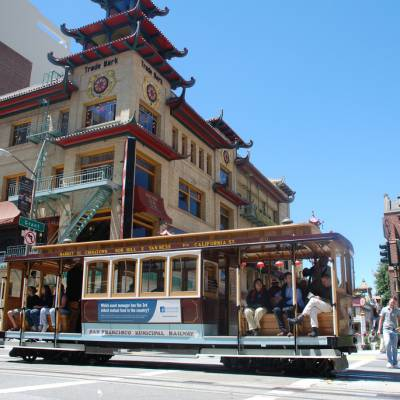
\includegraphics[width=1\textwidth]{./images/lorem.jpeg}
%   \captionsetup{name=Abb.,font=footnotesize}
%   \caption{Beispiel bild und beispiel cite \supercite{WinNT}}
% \end{figure}

\newpage
%-------------------------------------------------------------------------------
% 2
%-------------------------------------------------------------------------------

\section{Vorgehensweise}
\subsection{Auswahl der Programmiersprache}

Ich habe mir für die Umsetzung des Praxisprojekts die Programmiersprache Go ausgewählt. \cite{GOLANG}
Das Hauptgeschäftsfeld des Unternehmens in dem ich mein Praxisprojekt umsetzte besteht in der Entwicklung und Administration von Cloud-Computing-Systemen. Daher lag der Schluß nahe eine Programmiersprache zu wählen die den Anforderungen des Cloud-Computings gerecht werden kann. Auch in Hinblick auf zukünftige Projekte in dem Unternehmen erschien mir das Erlernen dieser neuen Programmiersprache als sehr sinnvoll.

Go ist eine kompilierbare Programmiersprache, die Nebenläufigkeit unterstützt und über eine automatische Speicherbereinigung verfügt. Entwickelt wurde Go von Mitarbeitern des Unternehmens Google Inc. Sie wurde aus Unzufriedenheit über die bestehenden Sprachen zur Softwareentwicklung wie C++ oder Java im Kontext heutiger Computersysteme, insbesondere im Hinblick auf skalierbare Netzwerkdienste, Cluster- und Cloud Computing, entwickelt. Aufgrund der reduzierten Sprachmittel kann der Compiler rasend schnell den Quelltext übersetzen. Dadurch eignet sich Go gut für Einsatzbereiche, die sonst eher Skriptsprachen vorbehalten sind. Die folgende Grafik soll die Effizienz und Einfachheit der Sprache verdeutlichen.

% \begin{figure}[!htp]
% 	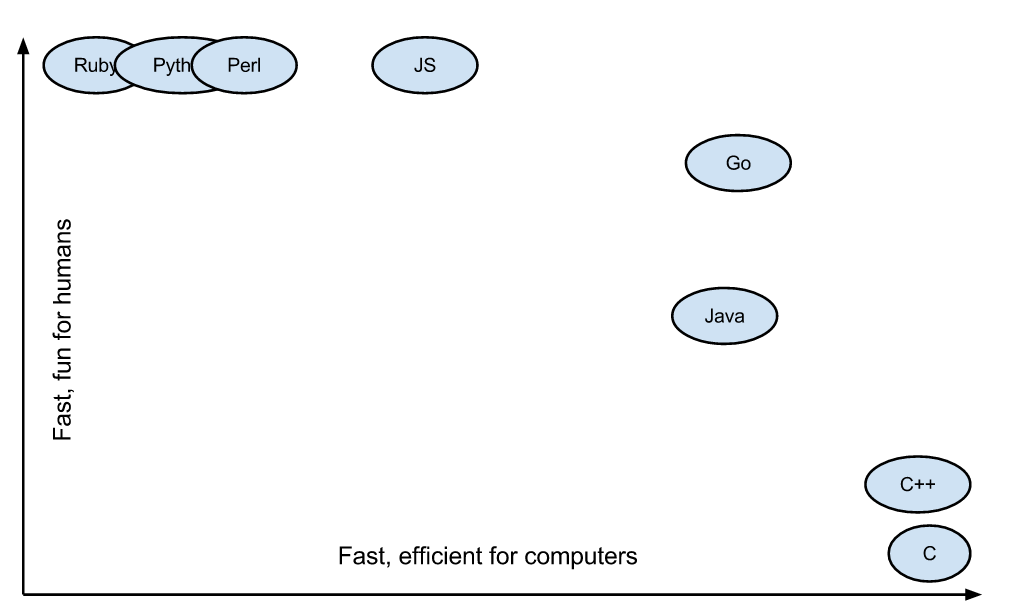
\includegraphics[width=1\textwidth]{images/golang_humans_computers.png}
% 	\captionsetup{name=Abb.,font=footnotesize}
% 	\caption{Code-Lesbarkeit und Effizienz}
% \end{figure}

% \begin{figure}[h!]
%   \centering     %%% not \center
%   \subfigure[Grauwertbild]{\label{fig:a}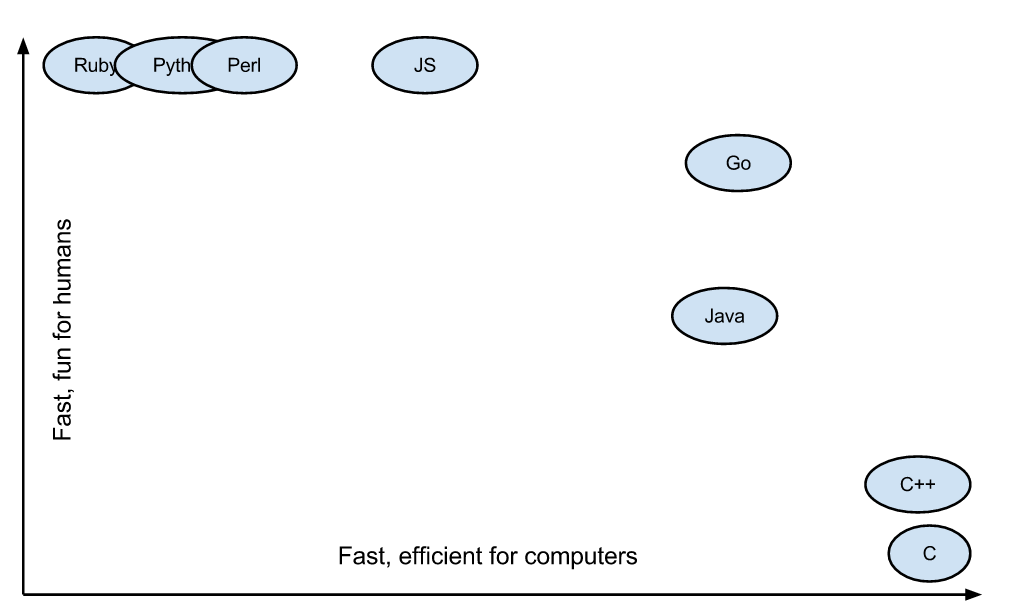
\includegraphics[width=0.5\textwidth]{images/golang_humans_computers.png}}
%   \subfigure[mathematisches Modell]{\label{fig:b}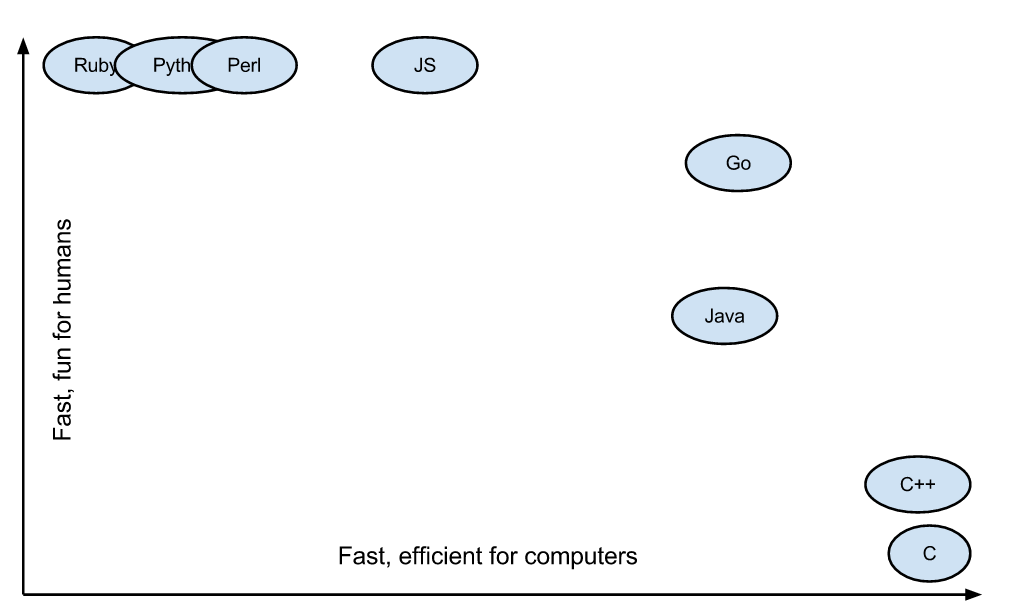
\includegraphics[width=0.5\textwidth]{images/golang_humans_computers.png}}
%   \caption{Überführung eines Bildes in ein mathematisches Modell (Datenstruktur).}
% \end{figure}

\begin{figure}[h!]
\centering
\subcaptionbox{Code-Lesbarkeit und Effizienz}{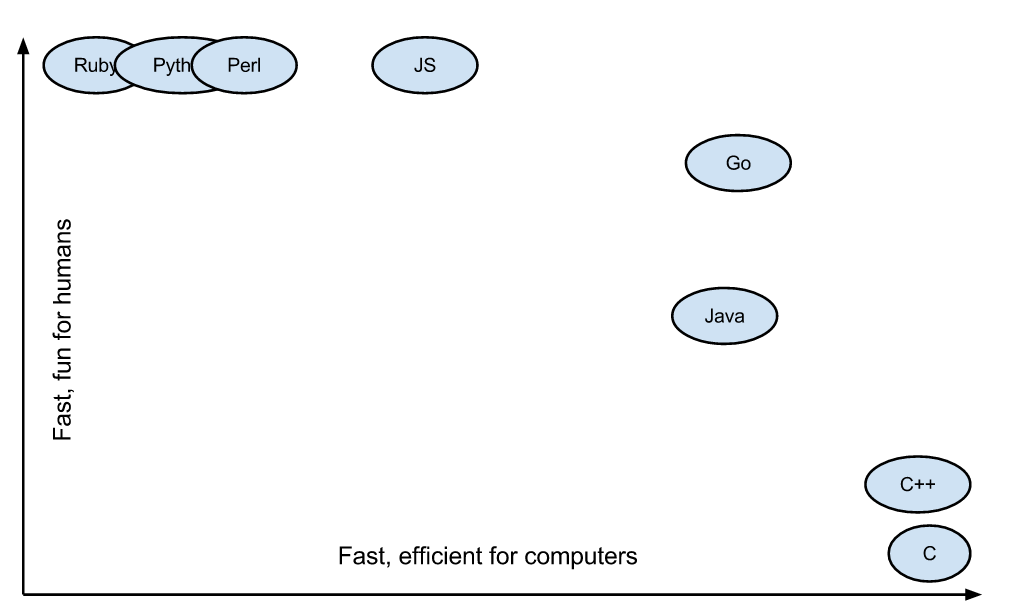
\includegraphics[width=0.45\textwidth]{images/golang_humans_computers.png}}%
\hfill
\subcaptionbox{Code-Lesbarkeit und Nebenläufigkeit}{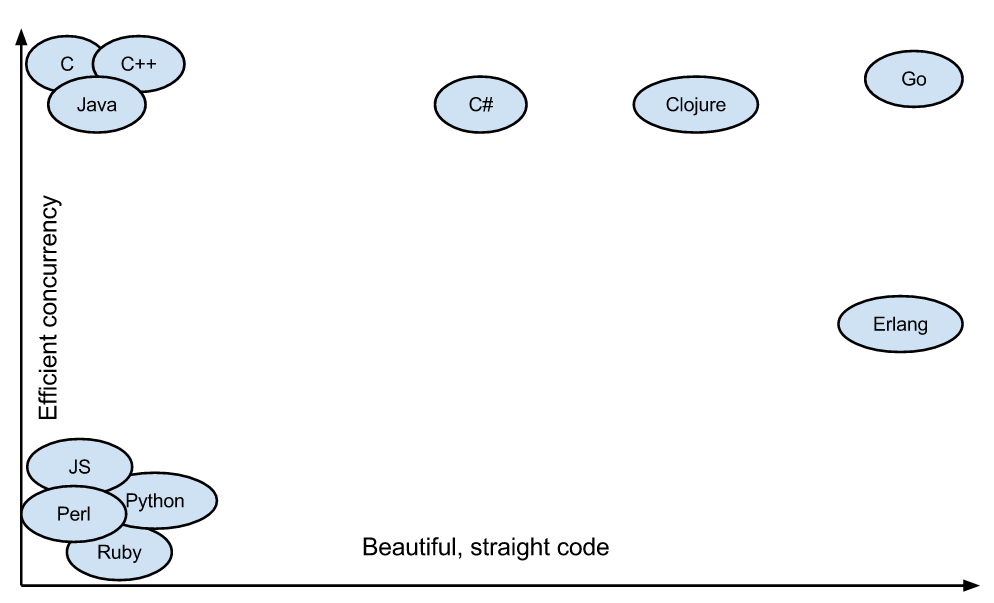
\includegraphics[width=0.45\textwidth]{images/golang_eff_concurrency_straightcode.png}}%
\hfill
\caption{Vorteile von Golang gegenüber anderen Programmiersprachen.}
\end{figure}


Die oben aufgeführten Sprachmerkmale haben dazu geführt das ich für mein Praxisprojekt die Programmiersprache Go ausgewählt habe. Go verfügt über eine saubere Syntax mit textbasiertem Workflow, minimalistischem Design und klarer Sprachspezifikation. So war es mir möglich die Sprache schnell zu erlernen und produktiv zu werden. Die Einfachheit der Sprache vereinfachte auch die Wartbarkeit des Codes und beschleunigte den Entwicklungsprozess. Ein wichtiges Sprachmerkmal von Go ist Geschwindigkeit einer kompilierten Sprache, aber das Gefühl einer interpretierten Sprache.

\subsection{Wichtige Technologien}

In diesem Abschnitt möchte ich wichtige Technologien benennen und vorstellen die mir bei der Umsetzung der Aufgabe geholfen haben.

\subsubsection{Versionskontrolle - Git}

Ein elementares Werkzeug stellte für mich die Versionskontrolle Git dar \cite{GIT}. Eine Versionskontrolle ermöglicht zum einen die Versionierung des Entwicklungsstandes aber auch das verteilte und kollaborative Arbeiten an einem Softwareprojekt.

Mit Git war es mir möglich den Quellcode über verschiedene Workstations hinweg verteilt zu bearbeiten (Distributed Version Control System). Als Remote habe ich den Quellcode in einem privaten Git-Repository auf github.com \cite{GITHUB} verwaltet.

Ich habe bei der Versionierung den Ansatz des Featurebranchings verfolgt (siehe Abbildung 2). Das bedeutet das man einen Master-Branch hat der stabil ist. Funktionalitäten werden in einem Entwicklungszweig (Branch) entwickelt und nach Vollendung mit dem Master gemerged. Dieser Ansatz ermöglichte mir eine nicht lineare Entwicklung , bestimmte Features auszuprobieren und nach Vollendung entweder in den Master zu mergen oder zu verwerfen.
% Der Ansatz des Branchings hat mir geholfen Entwicklungszweige zu nutzen und Features auszuprobieren die später in den Master gemerged wurden.

\begin{figure}[htp!]
  \centering
  \begin{tikzpicture}
    \matrix[row sep=20mm,column sep=40mm ,nodes={draw, thick, fill=black!20},
          row sep=1.2cm,column sep=0.5cm] {
      % Top Row (feature branch)
      & \node [rectangle] (feature) {Feature 1}; & \node[diamond] (c2) {2}; & \node[diamond] (c4) {4}; & \node[diamond] (c5) {5}; & & &\\
      % Middle Row (trunk)
      \node [rectangle] (trunk) {Master-Branch}; & \node[diamond] (c1) {1}; & \node[diamond] (c3) {3}; &  &  & \node[diamond] (c8) {8}; & \node [circle] (tend) {};\\
      % Bottom Row (feature branch 2)
      & & \node [rectangle] (feature2) {Feature 2}; & \node[diamond] (c6) {6}; & \node[diamond] (c7) {7}; &  & \node [circle] (f2end) {}; & &\\
    };
    \begin{scope}[every node/.style={midway,auto,font=\scriptsize}]
      \draw [very thick, ->] (trunk) -- (c1) -- (c3) -- (c8) -- (tend);
      \draw [very thick, ->] (feature) -- (c2) -- (c4) -- (c5);
      \draw [very thick, ->] (feature2) -- (c6) -- (c7) -- (f2end);
      \draw [dashed, very thick, ->] (trunk) -- node {$branch$} (feature);
      \draw [dashed, very thick, ->] (c1) -- node {$branch$} (feature2);
      \draw [dashed, very thick, ->] (c1) -- node {} (c2);
      \draw [dashed, very thick, ->] (c3) -- node {} (c4);
      \draw [dashed, very thick, ->] (c5) -- node {$merge$} (c8);
      \draw [dashed, very thick, ->] (c3) -- node {} (c6);
    \end{scope}
  \end{tikzpicture}

  \caption{Schematische Darstellung des Feature-Branching-Workflow}
  \label{}
\end{figure}


Darüberhinaus deckte die Arbeit mit Git auch die Anforderung an das Erfassen von Requirements ab. (Requirements-Engineering) Anforderungen wurden durch sogenannte Issue's direkt im Repository, sehr Quellcode nah erfasst, und bearbeitet. Über die Website github.com konnte auch direkt auf Quellcodestellen oder auf bestimmte Codeveränderungen (Commits) referenziert werden.

Eine Einbindung mehrerer Remotes (e.g. produktiv) zur Erstellung eines Deploymentprozesses ist dadurch auch möglich.




\subsubsection{Development und Deployment - Docker}

Ein weiteres sehr wichtiges Tool war die Containervirtualisierung Docker \cite{DOCKER}. Sie ersparte mir enorm viel Zeit mit dem Aufsetzen der komplexen Softwarearchitektur. Sie minderte den Konfigurationsaufwand und half mir bei der Integration der Abhängigkeiten des Softwaresystems mit dem Ziel den lokalen Stack so produktivnah wie möglich aufzusetzen. (siehe Abschnitt Architektur)

Docker ist eine Open-Source-Software zur Isolierung von Anwendungen mit Containervirtualisierung. Es vereinfacht die Bereitstellung von Anwendungen, weil sich Container, die alle nötigen Pakete enthalten, leicht als Dateien transportieren und installieren lassen (Dockerfile). Container gewährleisten die Trennung und Verwaltung der auf einem Rechner genutzten Ressourcen. Das beinhaltet laut Aussage der Entwickler: Code, Laufzeitmodul, Systemwerkzeuge, Systembibliotheken - alles was auf einem Rechner installiert werden kann.

Zur Orchestrierung der einzelnen Containeranwendung hab ich Docker-Compose verwendet. Docker-Compose ist ein Tool zum Definieren und Ausführen von Docker-Anwendungen mit mehreren Containern. Die Konfiguration der einzelnen Container wird in einem YAML-File, was in der Repo versioniert wird, beschrieben.

\bigbreak


\lstset{basicstyle=\ttfamily}
\lstset{xleftmargin=.2\textwidth, xrightmargin=.2\textwidth}
\begin{lstlisting}[language=yaml,frame=single]
version: '2'
services:
  mongodb:
    image: mongo:latest
    container_name: "mongodb"
    ports:
      - "27017:27017"
  minio1:
    image: minio/minio
    container_name: "minio"
    volumes:
      - ./data:/data
    ports:
      - "9001:9000"
    environment:
      MINIO_ACCESS_KEY: minio
      MINIO_SECRET_KEY: minio123
    command: server /data
\end{lstlisting}
\captionof{lstlisting}{Beispiel: Docker-Compose.yml zur Konfiguration von einer MongoDB-Datenbank und einem MinIO-Objectstore in einer Multicontainer-Architektur}



\subsubsection{Weitere wichtige Tools}

\subparagraph{Mermaid - Sequenzdiagram}

Als weiteres wichtiges Tool zur Modellierung des Prozessablaufes in einem Sequenzdiagramm ist das Tool Mermaid. Es arbeitet ähnlich wie Plant-UMl textbasiert und ist somit versionierbar. Damit war es mir möglich aus einem textbasiertem YAML ähnlichem Format ein Sequenzdiagramm zu rendern.

\subparagraph{Tmux}

\subparagraph{Tmuxinator}
\subparagraph{Rest-Clients / Insomia - Curl}

\newpage
\subsection{Umsetzung}

In diesem Abschnitt möchte ich in einer zeitlichen Reihenfolge die Tätigkeiten beschreiben die ich in meinem Praxisprojekt umgesetzt habe.

\paragraph{Kalenderwoche 41 - 42}\mbox{}\\

Die Anfangsphase war zum größten Teil eine Orientierungsphase. Ich habe mich in dieser Zeit auf die Programmiersprache Go festgelegt. Daher habe ich mich in dieser Phase habe vor allem mit der Einarbeitung in die Programmiersprache Go beschäftigt - Die Entwicklungsumgebung aufgesetzt und erste Schritte unternommen.

Ich habe mich viel mit dem Package http https://golang.org/pkg/net/http/ auseinandergesetzt. Erste Http Handler geschrieben und geeignete Pattern (Decorator) für die Umsetzung von Rest-Services ausprobiert.

\subparagraph{Kalenderwoche 43 - 44}\mbox{}\\

Hier habe ich den Beschluss gefasst kein Framework zu verwenden, sondern eher auf Bibliotheken zurückzugreifen. Die Verwendung von Bibliotheken hat den Vorteil mehr Kontrolle in der Entwicklung des Projekts zu haben. Der Unterschied zwischen einer Bibliothek und einem Framework liegt in dem Ansatz des \textit{Inversion of Controls}.

\textit{Inversion von Control} ist ein wichtiger Teil dessen, was ein Framework von einer Bibliothek unterscheidet. Eine Bibliothek ist im Wesentlichen eine Reihe von Funktionen, welche normalerweise klassenorientiert aufgerufen werden können. Die Kontrolle über den Aufruf liegt beim Client.

Ein Framework hingegen verkörpert ein abstrakteres Design mit mehr eingebautem Verhalten. Um ein Framework verwenden zu können, muss das Verhalten an verschiedenen Stellen im Framework eingefügt werden, entweder durch Unterklassenbildung oder durch das Injezieren eigener Klassen. Der Code des Frameworks ruft dann den Code an diesen Punkten auf. Die Kontrolle liegt also beim Framework.

In dieser Phase habe ich mich auch viel mit der Umsetung des Routing der API auseinandergesetzt. Ich habe dazu die Bibliothek  (https://github.com/gorilla/mux) ausgewählt um das Routing in der Rest-Api umzusetzen.
Dann habe ich versucht einen ersten einfachen Prototypen einer Rest-Api zu entwickeln. Der Prototyp beinhaltet lediglich einfache HTTP-Requests ohne weiterer Funktionalität.

Desweiteren habe ich mich mit dem in Go fest integriertem Unit-Test-Framework (https://golang.org/pkg/testing/) auseinandergesetzt und mich mit den Ansätzen des TDD (Test Driven Development) beschäftigt.

Ein weiterer Entschluss den ich in dieser Phase gefasst habe, war die Authentifizierung der API in einen Service auszulagern. Der Zugriff auf die Api erfolgt über ein Api-Gateway was die Authentifizierung und Authorisierung regelt. (siehe Architektur: Kong - Api - Gateway).

\subparagraph{Kalenderwoche 45 - 46}\mbox{}\\

In diesem Abschnitt des Praxisprojekts habe ich zunächst ein Refactoring der Projektstruktur vollzogen und mich versucht an das Standard Layout eines Go-Projektes zu halten. Die Spezifikationen zum Project Layout habe ich auf folgender Website ermittelt. (https://github.com/golang-standards/project-layout) (siehe Abbildung 3)
\bigbreak
\renewcommand*\DTstylecomment{\rmfamily\color{red}\textsc}
\begin{figure}[h!]
\centering
\framebox[\textwidth]{%
\begin{minipage}{0.9\textwidth}
\dirtree{%
.1 / .
.2 cmd .
	.3 server .
		.4 hpc-rest-api.go .
.2 src .
	.3 connection .
		.4 config.go .
	.3 handler .
		.4 authhandler.go .
		.4 jobhandler.go .
		.4 templatehandler.go .
		.4 logginghandler.go .
	.3 repository .
		.4 jobrepository.go .
		.4 templaterepository.go .
	.3 router .
		.4 router.go .
}

\end{minipage}
}
\caption{Projektstruktur der Rest-Api}
\end{figure}

\bigbreak
Des weiteren habe ich mich konzeptionell mit der High-Level-Architektur der Api befasst (siehe Abbildung 4). In dieser Phase habe ich ein Konzept für den Prozessablauf - das Submitten eines Jobs durch die Api - entwickelt. Ich habe dazu die Anforderungen an die Rest-Api spezifiziert und notwendige Api-Endpoints definiert.

Im Zuge dessen habe ich mit verschiedenen Technologien auseinandergesetzt die für diese Anforderungen notwendig sind. Zum Beispiel sollte der Consumer der Api eine Möglichkeit bekommen für den Job notwendige Files hochzuladen. Diese Files und die aus den Parametern des Jobs ergebenen Konfigurationstemplates, welche die Variantensimulationen ermöglichen, sollen in einem Objectstore gespeichert werden.

Als Service für den Objectstore ich Minio ausgewählt und einen Prototypen zur Interaktion mit dem Objektstore entwickelt. Dazu habe ich auf die Minio-Go Bibliothek zurückgegriffen und einen einfachen FileUploader über diesen Client entwickelt. (https://github.com/minio/minio-go.)

Auf der Solver - Layer, der hintersten Ebene die das Cluster-Backend darstellen soll, habe ich einen einfachen Job-Mock entwickelt der ein HPC-Job simulieren soll. Dieser Job wird innerhalb eines Docker-Containers ausgeführt und über Nomad - einem Job-Schedulling-Service mittels einer Queue verwaltet. Diese Phase meines Praxisprojekts war eher konzeptionell geprägt.

\begin{figure}[h!]
  \centering
  \begin{Verbatim}[fontsize=\tiny,frame=single]
                      +                                               +
  CLIENT_LAYER        |              API_LAYER                        |            SOLVER_LAYER
                      |                                               |
                      |                                               |
                      |                                               |
                      | Forward Requests                    Submit    |                           Submit Job
   +------------------+                   +--------------+            +----------------------+      Docker       +-------+
   | Kong Api Gateway +-----------------> | HPC-REST-API +----------> | NOMAD Job Scheduling +-----------------> | Node1 |
   | :8000            |                   | :7777        |            | :4646                |                   +-------+
   | :8001            |                   +--------------+            +----------------------+
   | :8443            |                    |                          |                                          +-------+
   | :8444            |                    |                          |                                          | Node2 |
   +------------------+                    | FILES                    |                                          +-------+
                      |                    |                          |
                      |                   +v------------------+       |                                          +-------+
                      |                   | MINIO Objectstore |       |                                          | Node3 |
                      |                   | :9001             |       |                                          +-------+
                      |                   | :9002             |       |
                      |                   | :9003             |       |                                          +-------+
                      |                   | :9004             |       |                                          | Node4 |
                      |                   +-------------------+       |                                          +-------+
                      |                                               |
  +----------------------------------------------------------------------------------------------------------------------+
                      |                                               |
  PERSISTENCE         |                                               |
                      |                                               |
   +------------------+                   +---------------------------+
   | POSTGRES         |                   | MongoDB                   |
   | :5432            |                   | :27017                    |
   +------------------+                   +---------------------------+
  \end{Verbatim}


  \caption{High-Level Architektur der Rest-Api \cite{WinNT}}
  \label{}
\end{figure}

\newpage
\subparagraph{Kalenderwoche 47 - 48}\mbox{}\\

In dieser Zeit habe ich mich vor allem mit der Implementierung der Endpoints befasst. Es können Jobs angelegt, ausgelesen, bearbeitet, und gelöscht werden. (CRUD - create,read,update,delete). Die Jobs werden in einer Mongo-Datenbank gespeichert. Dafür habe ich die Packages gopkg.in/mgo.v2 und gopkg.in/mgo.v2/bson verwendet. Die Jobs werden in einer Collection in der Mongo-Datenbank gespeichert. Zu jedem erzeugten Job ist es Möglich ein oder mehrere Templates anzulegen, welche die Varianten darstellen sollen. Als eindeutige Referenz zu der Job-Ressource dient die Unique Job-ID welche vom Datenbankschema erzeugt wird (bson.NewObjectId).

\begin{figure}[h!]
\resizebox{\textwidth}{!}{
\begin{tabular}{||l|r|l||}
	\hline
 \textbf{URI-Endpoint}  & \textbf{HTTP-Method} & \textbf{Description} \\ \hline\hline
 \texttt{/jobs/} & GET & Get all Jobs \\ \hline
 \texttt{/jobs/} & POST & Create new Job \\ \hline
 \texttt{/jobs/} & PUT & Update Job \\ \hline
 \texttt{/jobs/} & DELETE & Delete Job \\ \hline
 \texttt{/jobs/\{jobID\}} & GET & Get specific Job \\ \hline \hline
 \texttt{/jobs/\{jobID\}/templates/} & GET & Get all Templates \\ \hline
 \texttt{/jobs/\{jobID\}/templates/} & POST & Create new Template \\ \hline
 \texttt{/jobs/\{jobID\}/templates/} & PUT & Update Template \\ \hline
 \texttt{/jobs/\{jobID\}/templates/} & DELETE & Delete Template \\ \hline
 \texttt{/jobs/\{jobID\}/templates/\{templateID\}} & GET & Get specific Template \\ \hline
\end{tabular}
}
\caption{Api Endpoints (Job \& Template - Ressource)}
\label{tab:meinetabelle}
\end{figure}

Desweiteren habe ich mich in dieser Phase mit Best-Practices zu Microservices-Architekturen beschäftigt. Ich habe mich mit Behaviour Driven Development beschäftigt.



\subparagraph{Kalenderwoche 49 - 02}\mbox{}\\

In der letzten Phase meines Praxisprojekts hab ich vor allem mit dem Job-Submit Prozess beschäftigt. (https://www.nomadproject.io/) Die Jobs werden über die Nomad-Api in eine Queue aufgenommen und mittels Consul in einem Docker-Container gestartet.

\begin{figure}[h!]
\resizebox{\textwidth}{!}{
\begin{tabular}{||l|r|l||}
	\hline
 \textbf{URI-Endpoint}  & \textbf{HTTP-Method} & \textbf{Description} \\ \hline\hline
 \texttt{/jobs/\{jobID\}/submit    \hspace{15ex}              } & GET & Submit specific Job \\ \hline
\end{tabular}
}
\caption{Job Submit Endpoint}
\label{tab:meinetabelle}
\end{figure}




\subsection{Probleme bei der Umsetzung}

Aufgrund der Komplexität der Architektur und der gegebenen Zeit war mir nur ein sehr hard-codierte Implementierung der Api möglich. Ich musste mich in sehr viele Technologien einarbeiten und konzeptionell sehr viel erarbeiten. Die Solver-Layer wurde sehr abstrakt gehalten. Sie war für mich nur schwer verständlich und die sich daraus ergebenen Spezifikationen der Templates. Daher habe ich den Entschluss gefasst den Job als Attrappe umzusetzen. (Job-Mock - Fibonacci)

Die Api kann benutzt werden um einen Fibonacci Job mit den in dem angelegten Job angegebenen Parametern zu starten. Die Api übermittelt die Daten an die Nomad-Api. Nomad startet den Job in einem Docker-Container.


\newpage
%-------------------------------------------------------------------------------
% 3
%-------------------------------------------------------------------------------

\section{Architektur}

In diesem Abschnitte möchte ich noch einmal näher auf die verwendeten Services-Technologien eingehen die für die Gesamtarchitektur der Api notwendig waren.

\subsection{Authentifizierung - Kong Api-Gateway}

Kong ist eine skalierbare Open-Source-API-Schicht (auch bekannt als API-Gateway oder API-Middleware).Das Gateway läuft vor der RESTful-API und kann um Plugins erweitert , die zusätzliche Funktionen und Services bieten, die über die Kernplattform hinausgehen. (siehe Abbildung 6)

\begin{figure}[h!]
  \centering
  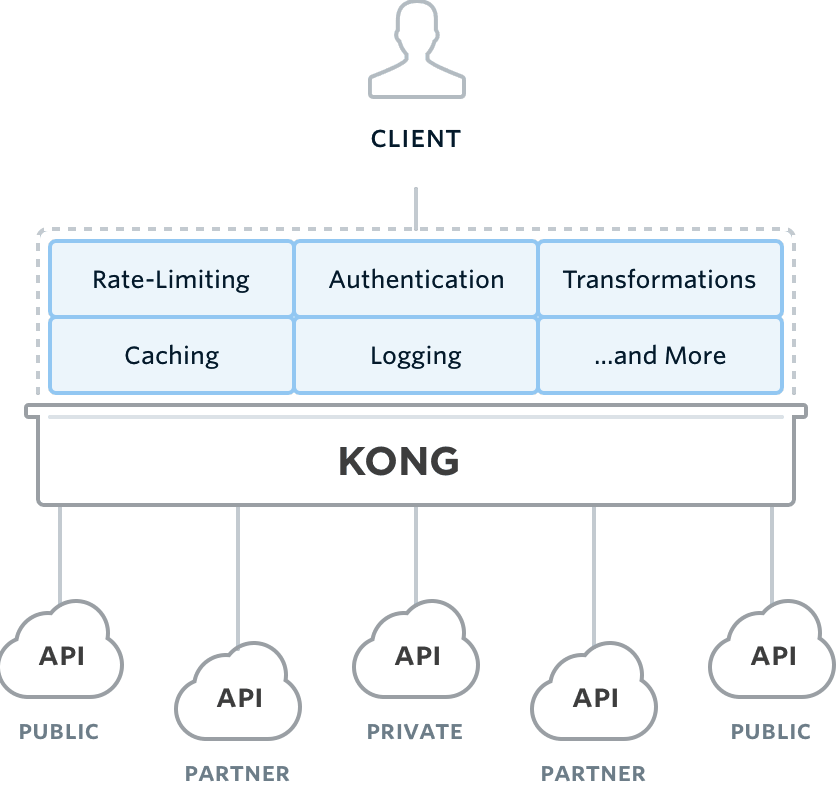
\includegraphics[width=0.5\textwidth]{images/kong_arch2.png}
  \caption{Kong Api-Gateway zur Authentifizierung}
  \label{}
\end{figure}

Kong habe ich als Authentifizierung für den Zugriff auf die Api benutzt.

% $ curl -i -X POST \
%   --url http://localhost:8001/apis/ \
%   --data 'name=example-api' \
%   --data 'hosts=example.com' \
%   --data 'upstream_url=http://mockbin.org'

\subsection{Persistenz - Mongo DB}

MongoDB (abgeleitet vom engl. humongous, „gigantisch“) ist eine dokumentenorientierte NoSQL-Datenbank, die in der Programmiersprache C++ geschrieben ist. Da die Datenbank dokumentenorientiert ist, kann sie Sammlungen von JSON-ähnlichen Dokumenten verwalten. So können viele Anwendungen Daten auf natürlichere Weise modellieren, da die Daten zwar in komplexen Hierarchien verschachtelt werden können, dabei aber immer abfragbar und indizierbar bleiben.

\subsection{Objectstore - Minio}

Minio ist ein Objektspeicherserver, der unter Apache License v2.0 veröffentlicht wurde. Es ist kompatibel mit Amazon S3 Cloud Storage Service. Es eignet sich am besten für die Speicherung unstrukturierter Daten wie Fotos, Videos, Protokolldateien, Backups und Container- / VM-Images. Die Größe eines Objekts kann zwischen einigen KB und maximal 5 TB liegen.

\subsection{Job Schedulling - Nomad}
Nomad is a single binary that schedules applications and services on Linux, Windows, and Mac. It is an open source scheduler that uses a declarative job file for scheduling virtualized, containerized, and standalone applications.


\newpage

%-------------------------------------------------------------------------------
% 4
%-------------------------------------------------------------------------------

\section{Schlusswort}


\newpage

\section{Zus"atzliche Informationen}
\subsection{Unternehmen}

CPU 24/7 ist spezialisiert auf die Vermietung und Administration
von High Performance Computing (HPC) Clustern.
Unsere Kunden sind Ingenieure, Maschinenbauer, Schiffsbauer und Autozulieferer.
Diese nutzen unsere Cluster um ihre 3D-Modelle in Physiksimulationen (Computer Aided Engineering, CAE)
zu optimieren und auf diese Weise die Entwicklungszeit von neuen Produkten zu reduzieren.

Webseite:\\
\url{https://www.cpu-24-7.com}



\subsection{Ansprechpersonen}

% \subsubsection{fachlich:}
% \texttt
\textbf{Richard Metzler M.Sc.}\\
Software Engineer Software Development\\

CPU 24/7 GmbH \\
August-Bebel-Stra"se 26-53\\
DE 14482 Potsdam\\

Telefon: +49 (0) 331 279 784 51 \\
E-Mail: r.metzler@cpu-24-7.com

% \subsubsection{organisatorisch:}
% \texttt
\bigbreak
\bigbreak
\textbf{Jenny Dawon M.A.}\\
Chief Administrative Officer (CAO)\\

CPU 24/7 GmbH\\
August-Bebel-Stra"se 26-53\\
DE 14482 Potsdam\\

Tel.: +49 (0) 331 279 784 44\\
E-Mail: j.dawon@cpu-24-7.com

\subsection{Ressourcen}
\textbf{Git-Repository als Versionskontrolle:}\\
\url{https://github.com/MatthiasHertel/ws17_pp}

\textbf{Webseite zur Dokumentation:}\\
\url{https://www.ws17-pp.mhertel.de}



%-------------------------------------------------------------------------------
% Literatur - Glossar - Akronyme
%-------------------------------------------------------------------------------
% \renewcommand\glossarytitle{}
\clearpage
\setlength\bibitemsep{10pt}
\renewcommand*{\bibfont}{\footnotesize}

\printbibliography[type=tech,heading=bibintoc, title=Verwendete Technologien]
\renewcommand*{\bibfont}{\footnotesize}
\printbibliography[type=package,heading=bibintoc, title=Verwendete Go-Packages]
\newpage
\phantomsection
\addcontentsline{toc}{section}{Abbildungsverzeichnis}
\listoffigures
\newpage

% \printglossary[type=\acronymtype, title=Abk"urzungsverzeichnis]
% \newpage
%
% \printglossary[type=main,title=Glossarverzeichnis]
% \newpage



%-------------------------------------------------------------------------------
% ENDE
%-------------------------------------------------------------------------------

\end{document}
